\documentclass[crop,border=7pt]{standalone}
\usepackage{tikz}
\usepackage{ifthen}
\usetikzlibrary{shapes.geometric}
\tikzset{
  hexagone/.style={
    draw, thick,
    fill=blue!20,
    shape=regular polygon,
    regular polygon sides=6,
    outer sep=0, inner sep=0,
    minimum size=1cm,
    %label={[red]center:#1}
  }
}
\begin{document}
  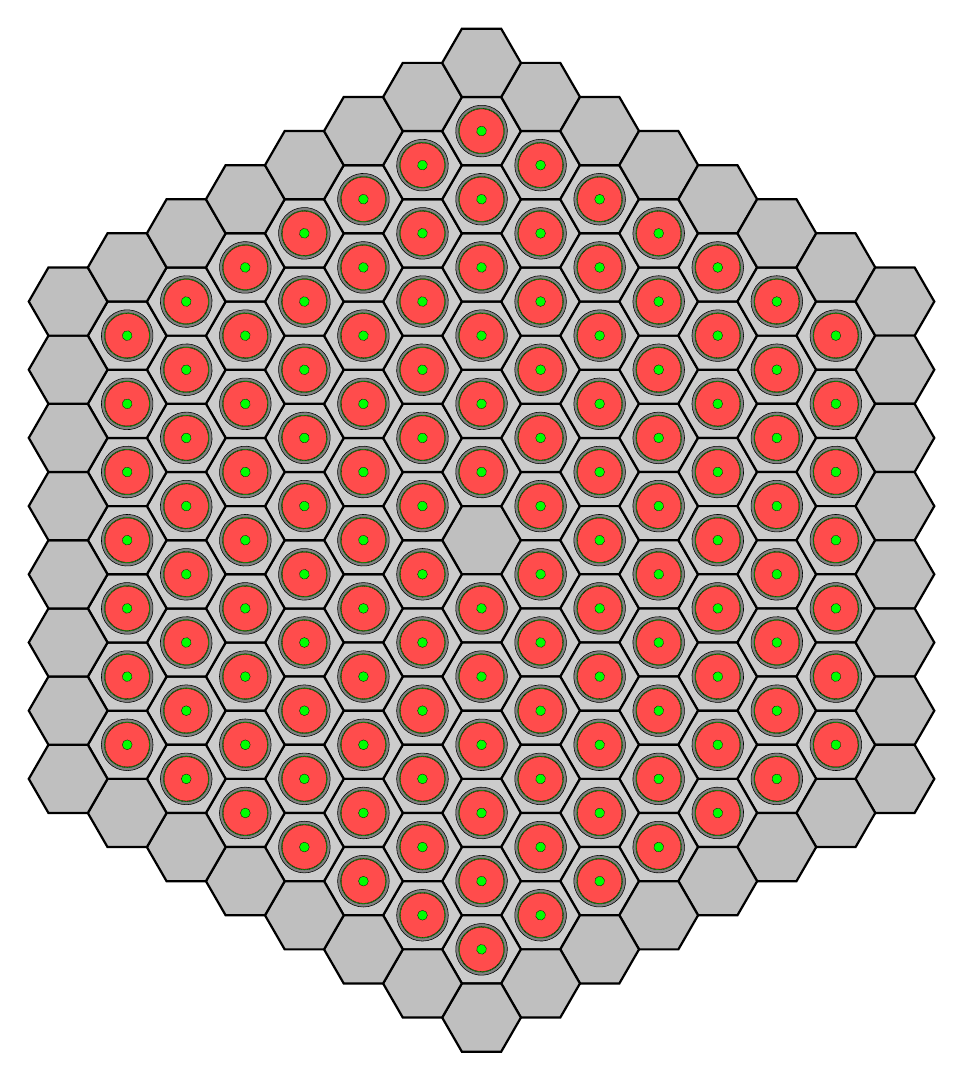
\begin{tikzpicture}
  
  %%%%%%%%%%%%%5
    \node[hexagone=0, fill=gray!50 ] at (0,0){};
    \foreach \r in {1,...,6}
      \foreach \t in {0,...,5}
        \foreach[evaluate={\l=int(\r*(\r-1)*3+\r*\t+\u)}] \u in {1,...,\r}
        \def\mycolor{gray!40}
          \scoped[rotate=-\t*60]
            \node[hexagone=\l, fill=\mycolor] at (0+.75*\u,{0.43301270189*(2*\r-\u)}){};
            
            
            
            
      \foreach \r in {7,...,7}
      \foreach \t in {0,...,5}
        \foreach[evaluate={\l=int(\r*(\r-1)*3+\r*\t+\u)}] \u in {1,...,\r}
        \def\mycolor{gray!50}
          \scoped[rotate=-\t*60]
            \node[hexagone=\l, fill=\mycolor] at (0+.75*\u,{0.43301270189*(2*\r-\u)}){};
   
  
  
%%%%%%%%%%%pins
  \foreach \r in {1,...,6}
      \foreach \t in {0,...,5}
        \foreach[evaluate={\l=int(\r*(\r-1)*3+\r*\t+\u)}] \u in {1,...,\r}
          \scoped[rotate=-\t*60]
% 	    \node[circle, fill=\mycolor] at (0+.75*\u,{0.43301270189*(2*\r-\u)}){};
	    \filldraw[gray, draw=black,very thin] (0+.75*\u,{0.43301270189*(2*\r-\u)}) circle (0.328cm);
	    
	    \foreach \r in {1,...,6}
      \foreach \t in {0,...,5}
        \foreach[evaluate={\l=int(\r*(\r-1)*3+\r*\t+\u)}] \u in {1,...,\r}
          \scoped[rotate=-\t*60]
% 	    \node[circle, fill=\mycolor] at (0+.75*\u,{0.43301270189*(2*\r-\u)}){};
	    \filldraw[green, draw=black, ultra thin] (0+.75*\u,{0.43301270189*(2*\r-\u)}) circle (0.290cm);
	
	
	\foreach \r in {1,...,6}    
  \foreach \t in {0,...,5}
        \foreach[evaluate={\l=int(\r*(\r-1)*3+\r*\t+\u)}] \u in {1,...,\r}
          \scoped[rotate=-\t*60]
% 	    \node[circle, fill=\mycolor] at (0+.75*\u,{0.43301270189*(2*\r-\u)}){};
	    \filldraw[red!70, draw=black,ultra thin] (0+.75*\u,{0.43301270189*(2*\r-\u)}) circle (0.281cm);
	    
	    
	    \foreach \r in {1,...,6}   
  \foreach \t in {0,...,5}
        \foreach[evaluate={\l=int(\r*(\r-1)*3+\r*\t+\u)}] \u in {1,...,\r}
          \scoped[rotate=-\t*60]
% 	    \node[circle, fill=\mycolor] at (0+.75*\u,{0.43301270189*(2*\r-\u)}){};
	    \filldraw[green, draw=black, ultra thin] (0+.75*\u,{0.43301270189*(2*\r-\u)}) circle (0.0625cm);
  
  
  

  \end{tikzpicture}
\end{document}